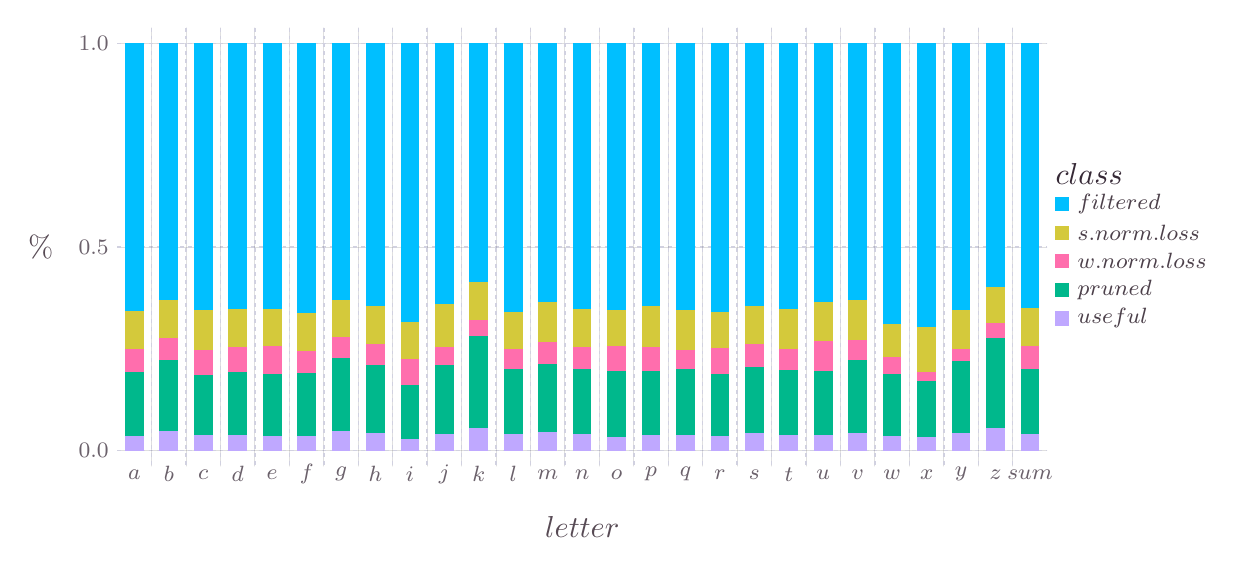
\begin{tikzpicture}[x=1mm,y=-1mm]
\definecolor{mycolorD4CA3A}{rgb}{0.83,0.79,0.23}
\definecolor{mycolor4C404B}{rgb}{0.3,0.25,0.29}
\definecolor{mycolor00BFFF}{rgb}{0,0.75,1}
\definecolor{mycolorD0D0E0}{rgb}{0.82,0.82,0.88}
\definecolor{mycolor362A35}{rgb}{0.21,0.16,0.21}
\definecolor{mycolor000000}{rgb}{0,0,0}
\definecolor{mycolor000000}{rgb}{0,0,0}
\definecolor{mycolor00B78D}{rgb}{0,0.72,0.55}
\definecolor{mycolor6C606B}{rgb}{0.42,0.38,0.42}
\definecolor{mycolorBEA9FF}{rgb}{0.75,0.66,1}
\definecolor{mycolorFF6DAE}{rgb}{1,0.43,0.68}
\definecolor{mycolor564A55}{rgb}{0.34,0.29,0.33}
\begin{scope}
\begin{scope}
\draw (77.07,68.39) node [text=mycolor564A55,draw=mycolor000000,draw opacity=0,rotate around={-0: (0,1.81)},inner sep=0.0]{\fontsize{3.88mm}{4.66mm}\selectfont $\text{letter}$};
\end{scope}
\begin{scope}
\draw (20.2,61.72) node [text=mycolor6C606B,rotate around={-0: (56.87,1.34)},inner sep=0.0]{\fontsize{2.82mm}{3.39mm}\selectfont $\text{a}$};
\draw (24.58,61.72) node [text=mycolor6C606B,rotate around={-0: (52.49,1.34)},inner sep=0.0]{\fontsize{2.82mm}{3.39mm}\selectfont $\text{b}$};
\draw (28.95,61.72) node [text=mycolor6C606B,rotate around={-0: (48.12,1.34)},inner sep=0.0]{\fontsize{2.82mm}{3.39mm}\selectfont $\text{c}$};
\draw (33.33,61.72) node [text=mycolor6C606B,rotate around={-0: (43.74,1.34)},inner sep=0.0]{\fontsize{2.82mm}{3.39mm}\selectfont $\text{d}$};
\draw (37.7,61.72) node [text=mycolor6C606B,rotate around={-0: (39.37,1.34)},inner sep=0.0]{\fontsize{2.82mm}{3.39mm}\selectfont $\text{e}$};
\draw (42.08,61.72) node [text=mycolor6C606B,rotate around={-0: (35,1.34)},inner sep=0.0]{\fontsize{2.82mm}{3.39mm}\selectfont $\text{f}$};
\draw (46.45,61.72) node [text=mycolor6C606B,rotate around={-0: (30.62,1.34)},inner sep=0.0]{\fontsize{2.82mm}{3.39mm}\selectfont $\text{g}$};
\draw (50.83,61.72) node [text=mycolor6C606B,rotate around={-0: (26.25,1.34)},inner sep=0.0]{\fontsize{2.82mm}{3.39mm}\selectfont $\text{h}$};
\draw (55.2,61.72) node [text=mycolor6C606B,rotate around={-0: (21.87,1.34)},inner sep=0.0]{\fontsize{2.82mm}{3.39mm}\selectfont $\text{i}$};
\draw (59.57,61.72) node [text=mycolor6C606B,rotate around={-0: (17.5,1.34)},inner sep=0.0]{\fontsize{2.82mm}{3.39mm}\selectfont $\text{j}$};
\draw (63.95,61.72) node [text=mycolor6C606B,rotate around={-0: (13.12,1.34)},inner sep=0.0]{\fontsize{2.82mm}{3.39mm}\selectfont $\text{k}$};
\draw (68.32,61.72) node [text=mycolor6C606B,rotate around={-0: (8.75,1.34)},inner sep=0.0]{\fontsize{2.82mm}{3.39mm}\selectfont $\text{l}$};
\draw (72.7,61.72) node [text=mycolor6C606B,rotate around={-0: (4.37,1.34)},inner sep=0.0]{\fontsize{2.82mm}{3.39mm}\selectfont $\text{m}$};
\draw (77.07,61.72) node [text=mycolor6C606B,rotate around={-0: (0,1.34)},inner sep=0.0]{\fontsize{2.82mm}{3.39mm}\selectfont $\text{n}$};
\draw (81.45,61.72) node [text=mycolor6C606B,rotate around={-0: (-4.37,1.34)},inner sep=0.0]{\fontsize{2.82mm}{3.39mm}\selectfont $\text{o}$};
\draw (85.82,61.72) node [text=mycolor6C606B,rotate around={-0: (-8.75,1.34)},inner sep=0.0]{\fontsize{2.82mm}{3.39mm}\selectfont $\text{p}$};
\draw (90.2,61.72) node [text=mycolor6C606B,rotate around={-0: (-13.12,1.34)},inner sep=0.0]{\fontsize{2.82mm}{3.39mm}\selectfont $\text{q}$};
\draw (94.57,61.72) node [text=mycolor6C606B,rotate around={-0: (-17.5,1.34)},inner sep=0.0]{\fontsize{2.82mm}{3.39mm}\selectfont $\text{r}$};
\draw (98.94,61.72) node [text=mycolor6C606B,rotate around={-0: (-21.87,1.34)},inner sep=0.0]{\fontsize{2.82mm}{3.39mm}\selectfont $\text{s}$};
\draw (103.32,61.72) node [text=mycolor6C606B,rotate around={-0: (-26.25,1.34)},inner sep=0.0]{\fontsize{2.82mm}{3.39mm}\selectfont $\text{t}$};
\draw (107.69,61.72) node [text=mycolor6C606B,rotate around={-0: (-30.62,1.34)},inner sep=0.0]{\fontsize{2.82mm}{3.39mm}\selectfont $\text{u}$};
\draw (112.07,61.72) node [text=mycolor6C606B,rotate around={-0: (-35,1.34)},inner sep=0.0]{\fontsize{2.82mm}{3.39mm}\selectfont $\text{v}$};
\draw (116.44,61.72) node [text=mycolor6C606B,rotate around={-0: (-39.37,1.34)},inner sep=0.0]{\fontsize{2.82mm}{3.39mm}\selectfont $\text{w}$};
\draw (120.82,61.72) node [text=mycolor6C606B,rotate around={-0: (-43.74,1.34)},inner sep=0.0]{\fontsize{2.82mm}{3.39mm}\selectfont $\text{x}$};
\draw (125.19,61.72) node [text=mycolor6C606B,rotate around={-0: (-48.12,1.34)},inner sep=0.0]{\fontsize{2.82mm}{3.39mm}\selectfont $\text{y}$};
\draw (129.57,61.72) node [text=mycolor6C606B,rotate around={-0: (-52.49,1.34)},inner sep=0.0]{\fontsize{2.82mm}{3.39mm}\selectfont $\text{z}$};
\draw (133.94,61.72) node [text=mycolor6C606B,rotate around={-0: (-56.87,1.34)},inner sep=0.0]{\fontsize{2.82mm}{3.39mm}\selectfont $\text{sum}$};
\end{scope}
\begin{scope}
\begin{scope}
\draw (139.94,27.42) node [text=mycolor4C404B,rotate around={-0: (5.62,5.44)},right,inner sep=0.0]{\fontsize{2.82mm}{3.39mm}\selectfont $\text{filtered}$};
\draw (139.94,31.04) node [text=mycolor4C404B,rotate around={-0: (5.62,1.81)},right,inner sep=0.0]{\fontsize{2.82mm}{3.39mm}\selectfont $\text{s.norm. loss}$};
\draw (139.94,34.67) node [text=mycolor4C404B,rotate around={-0: (5.62,-1.81)},right,inner sep=0.0]{\fontsize{2.82mm}{3.39mm}\selectfont $\text{w.norm. loss}$};
\draw (139.94,38.3) node [text=mycolor4C404B,rotate around={-0: (5.62,-5.44)},right,inner sep=0.0]{\fontsize{2.82mm}{3.39mm}\selectfont $\text{pruned}$};
\draw (139.94,41.92) node [text=mycolor4C404B,rotate around={-0: (5.62,-9.07)},right,inner sep=0.0]{\fontsize{2.82mm}{3.39mm}\selectfont $\text{useful}$};
\end{scope}
\begin{scope}
\path [fill=mycolor00BFFF,draw=mycolor000000,draw opacity=0] (137.13,26.51) rectangle +(1.81,1.81);
\path [fill=mycolorD4CA3A,draw=mycolor000000,draw opacity=0] (137.13,30.14) rectangle +(1.81,1.81);
\path [fill=mycolorFF6DAE,draw=mycolor000000,draw opacity=0] (137.13,33.76) rectangle +(1.81,1.81);
\path [fill=mycolor00B78D,draw=mycolor000000,draw opacity=0] (137.13,37.39) rectangle +(1.81,1.81);
\path [fill=mycolorBEA9FF,draw=mycolor000000,draw opacity=0] (137.13,41.02) rectangle +(1.81,1.81);
\end{scope}
\begin{scope}
\draw (137.13,23.6) node [text=mycolor362A35,draw=mycolor000000,draw opacity=0,rotate around={-0: (9.44,0.19)},right,inner sep=0.0]{\fontsize{3.88mm}{4.66mm}\selectfont $\text{class}$};
\end{scope}
\end{scope}
\begin{scope}
\clip  (18.02,5) -- (136.13,5) -- (136.13,60.72) -- (18.02,60.72);
\begin{scope}
\clip  (18.02,5) -- (136.13,5) -- (136.13,60.72) -- (18.02,60.72);
\path [fill=mycolor000000,fill opacity=0,draw=mycolor000000,draw opacity=0] (18.02,5) rectangle +(118.11,55.72);
\end{scope}
\begin{scope}
[dash pattern=on 0.5mm off 0.5mm,line width=0.2mm]
\path [fill=mycolor000000,draw=mycolorD0D0E0]  (18.02,58.72) -- (136.13,58.72);
\path [fill=mycolor000000,draw=mycolorD0D0E0]  (18.02,32.86) -- (136.13,32.86);
\path [fill=mycolor000000,draw=mycolorD0D0E0]  (18.02,7) -- (136.13,7);
\end{scope}
\begin{scope}
[dash pattern=on 0.5mm off 0.5mm,line width=0.2mm]
\path [fill=mycolor000000,draw=mycolorD0D0E0]  (22.39,5) -- (22.39,60.72);
\path [fill=mycolor000000,draw=mycolorD0D0E0]  (26.77,5) -- (26.77,60.72);
\path [fill=mycolor000000,draw=mycolorD0D0E0]  (31.14,5) -- (31.14,60.72);
\path [fill=mycolor000000,draw=mycolorD0D0E0]  (35.52,5) -- (35.52,60.72);
\path [fill=mycolor000000,draw=mycolorD0D0E0]  (39.89,5) -- (39.89,60.72);
\path [fill=mycolor000000,draw=mycolorD0D0E0]  (44.26,5) -- (44.26,60.72);
\path [fill=mycolor000000,draw=mycolorD0D0E0]  (48.64,5) -- (48.64,60.72);
\path [fill=mycolor000000,draw=mycolorD0D0E0]  (53.01,5) -- (53.01,60.72);
\path [fill=mycolor000000,draw=mycolorD0D0E0]  (57.39,5) -- (57.39,60.72);
\path [fill=mycolor000000,draw=mycolorD0D0E0]  (61.76,5) -- (61.76,60.72);
\path [fill=mycolor000000,draw=mycolorD0D0E0]  (66.14,5) -- (66.14,60.72);
\path [fill=mycolor000000,draw=mycolorD0D0E0]  (70.51,5) -- (70.51,60.72);
\path [fill=mycolor000000,draw=mycolorD0D0E0]  (74.88,5) -- (74.88,60.72);
\path [fill=mycolor000000,draw=mycolorD0D0E0]  (79.26,5) -- (79.26,60.72);
\path [fill=mycolor000000,draw=mycolorD0D0E0]  (83.63,5) -- (83.63,60.72);
\path [fill=mycolor000000,draw=mycolorD0D0E0]  (88.01,5) -- (88.01,60.72);
\path [fill=mycolor000000,draw=mycolorD0D0E0]  (92.38,5) -- (92.38,60.72);
\path [fill=mycolor000000,draw=mycolorD0D0E0]  (96.76,5) -- (96.76,60.72);
\path [fill=mycolor000000,draw=mycolorD0D0E0]  (101.13,5) -- (101.13,60.72);
\path [fill=mycolor000000,draw=mycolorD0D0E0]  (105.51,5) -- (105.51,60.72);
\path [fill=mycolor000000,draw=mycolorD0D0E0]  (109.88,5) -- (109.88,60.72);
\path [fill=mycolor000000,draw=mycolorD0D0E0]  (114.25,5) -- (114.25,60.72);
\path [fill=mycolor000000,draw=mycolorD0D0E0]  (118.63,5) -- (118.63,60.72);
\path [fill=mycolor000000,draw=mycolorD0D0E0]  (123,5) -- (123,60.72);
\path [fill=mycolor000000,draw=mycolorD0D0E0]  (127.38,5) -- (127.38,60.72);
\path [fill=mycolor000000,draw=mycolorD0D0E0]  (131.75,5) -- (131.75,60.72);
\end{scope}
\begin{scope}
\begin{scope}
[line width=0.3mm]
\begin{scope}
\path [fill=mycolorBEA9FF,draw=mycolor000000,draw opacity=0] (19.02,56.82) rectangle +(2.37,1.89);
\path [fill=mycolorBEA9FF,draw=mycolor000000,draw opacity=0] (23.39,56.26) rectangle +(2.37,2.46);
\path [fill=mycolorBEA9FF,draw=mycolor000000,draw opacity=0] (27.77,56.73) rectangle +(2.37,1.99);
\path [fill=mycolorBEA9FF,draw=mycolor000000,draw opacity=0] (32.14,56.7) rectangle +(2.37,2.01);
\path [fill=mycolorBEA9FF,draw=mycolor000000,draw opacity=0] (36.52,56.87) rectangle +(2.37,1.84);
\path [fill=mycolorBEA9FF,draw=mycolor000000,draw opacity=0] (40.89,56.81) rectangle +(2.37,1.9);
\path [fill=mycolorBEA9FF,draw=mycolor000000,draw opacity=0] (45.26,56.26) rectangle +(2.37,2.46);
\path [fill=mycolorBEA9FF,draw=mycolor000000,draw opacity=0] (49.64,56.46) rectangle +(2.37,2.26);
\path [fill=mycolorBEA9FF,draw=mycolor000000,draw opacity=0] (54.01,57.27) rectangle +(2.37,1.45);
\path [fill=mycolorBEA9FF,draw=mycolor000000,draw opacity=0] (58.39,56.61) rectangle +(2.37,2.1);
\path [fill=mycolorBEA9FF,draw=mycolor000000,draw opacity=0] (62.76,55.79) rectangle +(2.37,2.92);
\path [fill=mycolorBEA9FF,draw=mycolor000000,draw opacity=0] (67.14,56.62) rectangle +(2.37,2.09);
\path [fill=mycolorBEA9FF,draw=mycolor000000,draw opacity=0] (71.51,56.36) rectangle +(2.37,2.36);
\path [fill=mycolorBEA9FF,draw=mycolor000000,draw opacity=0] (75.88,56.56) rectangle +(2.37,2.16);
\path [fill=mycolorBEA9FF,draw=mycolor000000,draw opacity=0] (80.26,56.98) rectangle +(2.37,1.74);
\path [fill=mycolorBEA9FF,draw=mycolor000000,draw opacity=0] (84.63,56.69) rectangle +(2.37,2.03);
\path [fill=mycolorBEA9FF,draw=mycolor000000,draw opacity=0] (89.01,56.74) rectangle +(2.37,1.97);
\path [fill=mycolorBEA9FF,draw=mycolor000000,draw opacity=0] (93.38,56.8) rectangle +(2.37,1.91);
\path [fill=mycolorBEA9FF,draw=mycolor000000,draw opacity=0] (97.76,56.52) rectangle +(2.37,2.19);
\path [fill=mycolorBEA9FF,draw=mycolor000000,draw opacity=0] (102.13,56.73) rectangle +(2.37,1.98);
\path [fill=mycolorBEA9FF,draw=mycolor000000,draw opacity=0] (106.51,56.73) rectangle +(2.37,1.99);
\path [fill=mycolorBEA9FF,draw=mycolor000000,draw opacity=0] (110.88,56.52) rectangle +(2.37,2.19);
\path [fill=mycolorBEA9FF,draw=mycolor000000,draw opacity=0] (115.25,56.8) rectangle +(2.37,1.91);
\path [fill=mycolorBEA9FF,draw=mycolor000000,draw opacity=0] (119.63,56.98) rectangle +(2.37,1.74);
\path [fill=mycolorBEA9FF,draw=mycolor000000,draw opacity=0] (124,56.46) rectangle +(2.37,2.26);
\path [fill=mycolorBEA9FF,draw=mycolor000000,draw opacity=0] (128.38,55.85) rectangle +(2.37,2.86);
\path [fill=mycolorBEA9FF,draw=mycolor000000,draw opacity=0] (132.75,56.64) rectangle +(2.37,2.08);
\path [fill=mycolor00B78D,draw=mycolor000000,draw opacity=0] (19.02,48.78) rectangle +(2.37,8.04);
\path [fill=mycolor00B78D,draw=mycolor000000,draw opacity=0] (23.39,47.19) rectangle +(2.37,9.07);
\path [fill=mycolor00B78D,draw=mycolor000000,draw opacity=0] (27.77,49.08) rectangle +(2.37,7.65);
\path [fill=mycolor00B78D,draw=mycolor000000,draw opacity=0] (32.14,48.78) rectangle +(2.37,7.92);
\path [fill=mycolor00B78D,draw=mycolor000000,draw opacity=0] (36.52,49) rectangle +(2.37,7.87);
\path [fill=mycolor00B78D,draw=mycolor000000,draw opacity=0] (40.89,48.87) rectangle +(2.37,7.94);
\path [fill=mycolor00B78D,draw=mycolor000000,draw opacity=0] (45.26,47.01) rectangle +(2.37,9.24);
\path [fill=mycolor00B78D,draw=mycolor000000,draw opacity=0] (49.64,47.86) rectangle +(2.37,8.6);
\path [fill=mycolor00B78D,draw=mycolor000000,draw opacity=0] (54.01,50.39) rectangle +(2.37,6.88);
\path [fill=mycolor00B78D,draw=mycolor000000,draw opacity=0] (58.39,47.85) rectangle +(2.37,8.77);
\path [fill=mycolor00B78D,draw=mycolor000000,draw opacity=0] (62.76,44.21) rectangle +(2.37,11.58);
\path [fill=mycolor00B78D,draw=mycolor000000,draw opacity=0] (67.14,48.41) rectangle +(2.37,8.21);
\path [fill=mycolor00B78D,draw=mycolor000000,draw opacity=0] (71.51,47.73) rectangle +(2.37,8.63);
\path [fill=mycolor00B78D,draw=mycolor000000,draw opacity=0] (75.88,48.35) rectangle +(2.37,8.21);
\path [fill=mycolor00B78D,draw=mycolor000000,draw opacity=0] (80.26,48.64) rectangle +(2.37,8.34);
\path [fill=mycolor00B78D,draw=mycolor000000,draw opacity=0] (84.63,48.58) rectangle +(2.37,8.11);
\path [fill=mycolor00B78D,draw=mycolor000000,draw opacity=0] (89.01,48.33) rectangle +(2.37,8.41);
\path [fill=mycolor00B78D,draw=mycolor000000,draw opacity=0] (93.38,48.97) rectangle +(2.37,7.83);
\path [fill=mycolor00B78D,draw=mycolor000000,draw opacity=0] (97.76,48.04) rectangle +(2.37,8.48);
\path [fill=mycolor00B78D,draw=mycolor000000,draw opacity=0] (102.13,48.45) rectangle +(2.37,8.28);
\path [fill=mycolor00B78D,draw=mycolor000000,draw opacity=0] (106.51,48.64) rectangle +(2.37,8.09);
\path [fill=mycolor00B78D,draw=mycolor000000,draw opacity=0] (110.88,47.21) rectangle +(2.37,9.31);
\path [fill=mycolor00B78D,draw=mycolor000000,draw opacity=0] (115.25,48.95) rectangle +(2.37,7.86);
\path [fill=mycolor00B78D,draw=mycolor000000,draw opacity=0] (119.63,49.81) rectangle +(2.37,7.17);
\path [fill=mycolor00B78D,draw=mycolor000000,draw opacity=0] (124,47.36) rectangle +(2.37,9.1);
\path [fill=mycolor00B78D,draw=mycolor000000,draw opacity=0] (128.38,44.35) rectangle +(2.37,11.5);
\path [fill=mycolor00B78D,draw=mycolor000000,draw opacity=0] (132.75,48.31) rectangle +(2.37,8.33);
\path [fill=mycolorFF6DAE,draw=mycolor000000,draw opacity=0] (19.02,45.75) rectangle +(2.37,3.03);
\path [fill=mycolorFF6DAE,draw=mycolor000000,draw opacity=0] (23.39,44.4) rectangle +(2.37,2.79);
\path [fill=mycolorFF6DAE,draw=mycolor000000,draw opacity=0] (27.77,45.98) rectangle +(2.37,3.1);
\path [fill=mycolorFF6DAE,draw=mycolor000000,draw opacity=0] (32.14,45.55) rectangle +(2.37,3.23);
\path [fill=mycolorFF6DAE,draw=mycolor000000,draw opacity=0] (36.52,45.38) rectangle +(2.37,3.62);
\path [fill=mycolorFF6DAE,draw=mycolor000000,draw opacity=0] (40.89,46) rectangle +(2.37,2.87);
\path [fill=mycolorFF6DAE,draw=mycolor000000,draw opacity=0] (45.26,44.33) rectangle +(2.37,2.68);
\path [fill=mycolorFF6DAE,draw=mycolor000000,draw opacity=0] (49.64,45.21) rectangle +(2.37,2.64);
\path [fill=mycolorFF6DAE,draw=mycolor000000,draw opacity=0] (54.01,47.04) rectangle +(2.37,3.35);
\path [fill=mycolorFF6DAE,draw=mycolor000000,draw opacity=0] (58.39,45.57) rectangle +(2.37,2.28);
\path [fill=mycolorFF6DAE,draw=mycolor000000,draw opacity=0] (62.76,42.07) rectangle +(2.37,2.14);
\path [fill=mycolorFF6DAE,draw=mycolor000000,draw opacity=0] (67.14,45.85) rectangle +(2.37,2.56);
\path [fill=mycolorFF6DAE,draw=mycolor000000,draw opacity=0] (71.51,44.96) rectangle +(2.37,2.77);
\path [fill=mycolorFF6DAE,draw=mycolor000000,draw opacity=0] (75.88,45.56) rectangle +(2.37,2.78);
\path [fill=mycolorFF6DAE,draw=mycolor000000,draw opacity=0] (80.26,45.38) rectangle +(2.37,3.25);
\path [fill=mycolorFF6DAE,draw=mycolor000000,draw opacity=0] (84.63,45.51) rectangle +(2.37,3.07);
\path [fill=mycolorFF6DAE,draw=mycolor000000,draw opacity=0] (89.01,45.9) rectangle +(2.37,2.43);
\path [fill=mycolorFF6DAE,draw=mycolor000000,draw opacity=0] (93.38,45.65) rectangle +(2.37,3.32);
\path [fill=mycolorFF6DAE,draw=mycolor000000,draw opacity=0] (97.76,45.22) rectangle +(2.37,2.82);
\path [fill=mycolorFF6DAE,draw=mycolor000000,draw opacity=0] (102.13,45.83) rectangle +(2.37,2.63);
\path [fill=mycolorFF6DAE,draw=mycolor000000,draw opacity=0] (106.51,44.75) rectangle +(2.37,3.89);
\path [fill=mycolorFF6DAE,draw=mycolor000000,draw opacity=0] (110.88,44.63) rectangle +(2.37,2.58);
\path [fill=mycolorFF6DAE,draw=mycolor000000,draw opacity=0] (115.25,46.83) rectangle +(2.37,2.12);
\path [fill=mycolorFF6DAE,draw=mycolor000000,draw opacity=0] (119.63,48.69) rectangle +(2.37,1.12);
\path [fill=mycolorFF6DAE,draw=mycolor000000,draw opacity=0] (124,45.79) rectangle +(2.37,1.56);
\path [fill=mycolorFF6DAE,draw=mycolor000000,draw opacity=0] (128.38,42.47) rectangle +(2.37,1.88);
\path [fill=mycolorFF6DAE,draw=mycolor000000,draw opacity=0] (132.75,45.41) rectangle +(2.37,2.9);
\path [fill=mycolorD4CA3A,draw=mycolor000000,draw opacity=0] (19.02,40.99) rectangle +(2.37,4.76);
\path [fill=mycolorD4CA3A,draw=mycolor000000,draw opacity=0] (23.39,39.56) rectangle +(2.37,4.84);
\path [fill=mycolorD4CA3A,draw=mycolor000000,draw opacity=0] (27.77,40.91) rectangle +(2.37,5.07);
\path [fill=mycolorD4CA3A,draw=mycolor000000,draw opacity=0] (32.14,40.7) rectangle +(2.37,4.85);
\path [fill=mycolorD4CA3A,draw=mycolor000000,draw opacity=0] (36.52,40.71) rectangle +(2.37,4.68);
\path [fill=mycolorD4CA3A,draw=mycolor000000,draw opacity=0] (40.89,41.2) rectangle +(2.37,4.81);
\path [fill=mycolorD4CA3A,draw=mycolor000000,draw opacity=0] (45.26,39.54) rectangle +(2.37,4.79);
\path [fill=mycolorD4CA3A,draw=mycolor000000,draw opacity=0] (49.64,40.34) rectangle +(2.37,4.87);
\path [fill=mycolorD4CA3A,draw=mycolor000000,draw opacity=0] (54.01,42.33) rectangle +(2.37,4.71);
\path [fill=mycolorD4CA3A,draw=mycolor000000,draw opacity=0] (58.39,40.11) rectangle +(2.37,5.46);
\path [fill=mycolorD4CA3A,draw=mycolor000000,draw opacity=0] (62.76,37.27) rectangle +(2.37,4.8);
\path [fill=mycolorD4CA3A,draw=mycolor000000,draw opacity=0] (67.14,41.06) rectangle +(2.37,4.79);
\path [fill=mycolorD4CA3A,draw=mycolor000000,draw opacity=0] (71.51,39.88) rectangle +(2.37,5.08);
\path [fill=mycolorD4CA3A,draw=mycolor000000,draw opacity=0] (75.88,40.7) rectangle +(2.37,4.86);
\path [fill=mycolorD4CA3A,draw=mycolor000000,draw opacity=0] (80.26,40.81) rectangle +(2.37,4.57);
\path [fill=mycolorD4CA3A,draw=mycolor000000,draw opacity=0] (84.63,40.41) rectangle +(2.37,5.1);
\path [fill=mycolorD4CA3A,draw=mycolor000000,draw opacity=0] (89.01,40.88) rectangle +(2.37,5.02);
\path [fill=mycolorD4CA3A,draw=mycolor000000,draw opacity=0] (93.38,41.05) rectangle +(2.37,4.6);
\path [fill=mycolorD4CA3A,draw=mycolor000000,draw opacity=0] (97.76,40.3) rectangle +(2.37,4.92);
\path [fill=mycolorD4CA3A,draw=mycolor000000,draw opacity=0] (102.13,40.73) rectangle +(2.37,5.1);
\path [fill=mycolorD4CA3A,draw=mycolor000000,draw opacity=0] (106.51,39.82) rectangle +(2.37,4.92);
\path [fill=mycolorD4CA3A,draw=mycolor000000,draw opacity=0] (110.88,39.64) rectangle +(2.37,4.99);
\path [fill=mycolorD4CA3A,draw=mycolor000000,draw opacity=0] (115.25,42.61) rectangle +(2.37,4.22);
\path [fill=mycolorD4CA3A,draw=mycolor000000,draw opacity=0] (119.63,43) rectangle +(2.37,5.69);
\path [fill=mycolorD4CA3A,draw=mycolor000000,draw opacity=0] (124,40.89) rectangle +(2.37,4.9);
\path [fill=mycolorD4CA3A,draw=mycolor000000,draw opacity=0] (128.38,37.95) rectangle +(2.37,4.51);
\path [fill=mycolorD4CA3A,draw=mycolor000000,draw opacity=0] (132.75,40.54) rectangle +(2.37,4.87);
\path [fill=mycolor00BFFF,draw=mycolor000000,draw opacity=0] (19.02,7) rectangle +(2.37,33.99);
\path [fill=mycolor00BFFF,draw=mycolor000000,draw opacity=0] (23.39,7) rectangle +(2.37,32.56);
\path [fill=mycolor00BFFF,draw=mycolor000000,draw opacity=0] (27.77,7) rectangle +(2.37,33.91);
\path [fill=mycolor00BFFF,draw=mycolor000000,draw opacity=0] (32.14,7) rectangle +(2.37,33.7);
\path [fill=mycolor00BFFF,draw=mycolor000000,draw opacity=0] (36.52,7) rectangle +(2.37,33.71);
\path [fill=mycolor00BFFF,draw=mycolor000000,draw opacity=0] (40.89,7) rectangle +(2.37,34.2);
\path [fill=mycolor00BFFF,draw=mycolor000000,draw opacity=0] (45.26,7) rectangle +(2.37,32.54);
\path [fill=mycolor00BFFF,draw=mycolor000000,draw opacity=0] (49.64,7) rectangle +(2.37,33.34);
\path [fill=mycolor00BFFF,draw=mycolor000000,draw opacity=0] (54.01,7) rectangle +(2.37,35.33);
\path [fill=mycolor00BFFF,draw=mycolor000000,draw opacity=0] (58.39,7) rectangle +(2.37,33.11);
\path [fill=mycolor00BFFF,draw=mycolor000000,draw opacity=0] (62.76,7) rectangle +(2.37,30.27);
\path [fill=mycolor00BFFF,draw=mycolor000000,draw opacity=0] (67.14,7) rectangle +(2.37,34.06);
\path [fill=mycolor00BFFF,draw=mycolor000000,draw opacity=0] (71.51,7) rectangle +(2.37,32.88);
\path [fill=mycolor00BFFF,draw=mycolor000000,draw opacity=0] (75.88,7) rectangle +(2.37,33.7);
\path [fill=mycolor00BFFF,draw=mycolor000000,draw opacity=0] (80.26,7) rectangle +(2.37,33.81);
\path [fill=mycolor00BFFF,draw=mycolor000000,draw opacity=0] (84.63,7) rectangle +(2.37,33.41);
\path [fill=mycolor00BFFF,draw=mycolor000000,draw opacity=0] (89.01,7) rectangle +(2.37,33.88);
\path [fill=mycolor00BFFF,draw=mycolor000000,draw opacity=0] (93.38,7) rectangle +(2.37,34.05);
\path [fill=mycolor00BFFF,draw=mycolor000000,draw opacity=0] (97.76,7) rectangle +(2.37,33.3);
\path [fill=mycolor00BFFF,draw=mycolor000000,draw opacity=0] (102.13,7) rectangle +(2.37,33.73);
\path [fill=mycolor00BFFF,draw=mycolor000000,draw opacity=0] (106.51,7) rectangle +(2.37,32.82);
\path [fill=mycolor00BFFF,draw=mycolor000000,draw opacity=0] (110.88,7) rectangle +(2.37,32.64);
\path [fill=mycolor00BFFF,draw=mycolor000000,draw opacity=0] (115.25,7) rectangle +(2.37,35.61);
\path [fill=mycolor00BFFF,draw=mycolor000000,draw opacity=0] (119.63,7) rectangle +(2.37,36);
\path [fill=mycolor00BFFF,draw=mycolor000000,draw opacity=0] (124,7) rectangle +(2.37,33.89);
\path [fill=mycolor00BFFF,draw=mycolor000000,draw opacity=0] (128.38,7) rectangle +(2.37,30.95);
\path [fill=mycolor00BFFF,draw=mycolor000000,draw opacity=0] (132.75,7) rectangle +(2.37,33.54);
\end{scope}
\end{scope}
\end{scope}
\end{scope}
\begin{scope}
\draw (17.02,58.72) node [text=mycolor6C606B,rotate around={-0: (-2.01,-25.86)},left,inner sep=0.0]{\fontsize{2.82mm}{3.39mm}\selectfont $\text{0.0}$};
\draw (17.02,32.86) node [text=mycolor6C606B,rotate around={-0: (-2.01,-0)},left,inner sep=0.0]{\fontsize{2.82mm}{3.39mm}\selectfont $\text{0.5}$};
\draw (17.02,7) node [text=mycolor6C606B,rotate around={-0: (-2.01,25.86)},left,inner sep=0.0]{\fontsize{2.82mm}{3.39mm}\selectfont $\text{1.0}$};
\end{scope}
\begin{scope}
\draw (10,32.86) node [text=mycolor564A55,draw=mycolor000000,draw opacity=0,rotate around={-0: (-1.5,0)},left,inner sep=0.0]{\fontsize{3.88mm}{4.66mm}\selectfont $\text{\%}$};
\end{scope}
\end{scope}
\end{tikzpicture}
